\documentclass{beamer}

\usepackage[ruled]{algorithm2e}
\SetKw{KwRet}{return}
\SetKwRepeat{Repeat}{repeat}{until}
\usepackage{amsmath}

\usetheme{AnnArbor}
\usecolortheme{crane}
\usefonttheme[onlymath]{serif}

\title{Deep Learning - Foundations and Concepts}
\subtitle{Chapter 19. Autoencoders}
\author{nonlineark@github}
\date{\today}

\begin{document}

\begin{frame}
    \titlepage
\end{frame}

\begin{frame}
    \frametitle{Outline}
    \tableofcontents
\end{frame}

\section{Deterministic Autoencoders}

\begin{frame}
    \frametitle{Linear autoencoders}
    \begin{figure}
        \caption{An autoencoder neural network having two layers of weights}
        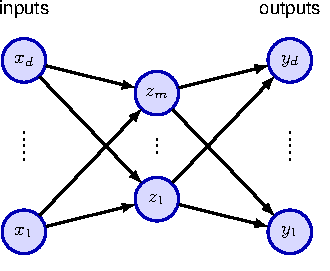
\includegraphics{Figure_1.pdf}
    \end{figure}
\end{frame}

\begin{frame}
    \frametitle{Linear autoencoders}
    Consider a two-layer neural network having $D$ inputs, $D$ output units and $M$ hidden units, with $M<D$. The targets used to train the network are simply the input vectors themselves, so that the network attempts to map each input vector onto itself. We choose a sum-of-squares error of the form:
    \begin{equation*}
        E(w)=\frac{1}{2}\sum_{n=1}^{N}||y(x_{n};w)-x_{n}||^{2}
    \end{equation*}
\end{frame}

\begin{frame}
    \frametitle{Linear autoencoders}
    \begin{itemize}
        \item If the hidden units have linear activation functions, then it can be shown that when the error function is minimized, the network performs a projection onto the $M$-dimensional subspace that is spanned by the first $M$ principal components of the data.
        \item Even with nonlinear hidden units, the minimum error solution is again given by the projection onto the principal component subspace. There is therefore no advantage in using two-layer neural networks to perform dimensionality reduction.
    \end{itemize}
\end{frame}

\begin{frame}
    \frametitle{Deep autoencoders}
    \begin{figure}
        \caption{A four-layer auto-associative network that can perform a nonlinear dimensionality reduction}
        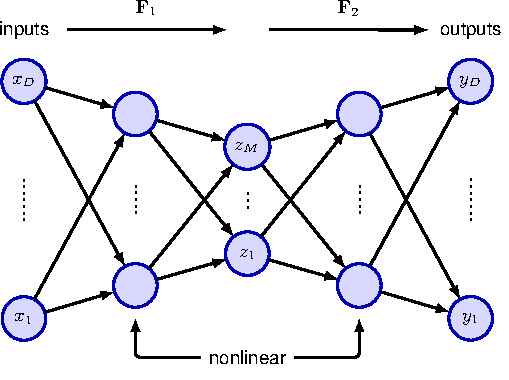
\includegraphics[height=0.6\textheight]{Figure_2.pdf}
    \end{figure}
\end{frame}

\begin{frame}
    \frametitle{Deep autoencoders}
    Consider the four-layer auto-associative network shown on the previous slide:
    \begin{itemize}
        \item The output units are linear, and the $M$ units in the second layer can also be linear.
        \item However, the first and third layers have sigmoidal nonlinear activation functions.
    \end{itemize}
    We can view this network as two successive functional mappings $F_{1}$ and $F_{2}$:
    \begin{itemize}
        \item $F_{1}$ projects the original $D$-dimensional data onto an $M$-dimensional subspace defined by the activations of the units in the second layer.
        \item $F_{2}$ maps from the $M$-dimensional hidden space back into the original $D$-dimensional input space.
    \end{itemize}
\end{frame}

\begin{frame}
    \frametitle{Deep autoencoders}
    \begin{itemize}
        \item Such a network effectively performs a nonlinear form of PCA.
        \item However:
        \begin{itemize}
            \item Training the network now involves a nonlinear optimization, and computationally intensive nonlinear optimization techniques must be used.
            \item There is the risk of finding a sub-optimal local minimum of the error function.
            \item The dimensionality of the subspace must be specified before training the network.
        \end{itemize}
    \end{itemize}
\end{frame}

\begin{frame}
    \frametitle{Sparse autoencoders}
    Instead of limiting the number of nodes in one of the hidden layers in the network, an alternative way to constrain the internal representation is to use a regularizer to encourage a sparse representation:
    \begin{equation*}
        \tilde{E}(w)=E(w)+\lambda\sum_{k=1}^{K}|z_{k}|
    \end{equation*}
    where $E(w)$ is the unregularized error, and the sum over $k$ is taken over the activation values of all the units in one of the hidden layers.
\end{frame}

\begin{frame}
    \frametitle{Denoising autoencoders}
    The idea of denoising autoencoders is to take each input vector $x_{n}$ and to corrupt it with noise to give a modified vector $\tilde{x}_{n}$ which is then input to an autoencoder to give an output $y(\tilde{x}_{n};w)$. The network is trained to reconstruct the original noise-free input vector:
    \begin{equation*}
        E(w)=\sum_{n=1}^{N}||y(\tilde{x}_{n};w)-x_{n}||^{2}
    \end{equation*}
\end{frame}

\begin{frame}
    \frametitle{Denoising autoencoders}
    \begin{itemize}
        \item One form of noise involves setting a randomly chosen subset of the input variables to zero.
        \item An alternative approach is to add independent zero-mean Gaussian noise to every input variable, where the scale of the noise is set by the variance of the Gaussian.
    \end{itemize}
\end{frame}

\begin{frame}
    \frametitle{Masked autoencoders}
    \begin{itemize}
        \item In a masked autoencoder, a deep network is used to reconstruct an image given a corrupted version of that image as input. The form of corruption is masking, or dropping out, part of the input image.
        \item This technique is generally used in combination with a vision transformer architecture.
        \item Compared to language, images have much more redundancy along with strong local correlations. The best internal representations are learned when a relatively high proportion of the input image is masked, typically $75\%$.
        \item The decoder is discarded and the encoder is applied to the full image with no masking and with a fresh set of output layers that are fine-tuned for the required application.
    \end{itemize}
\end{frame}

\begin{frame}
    \frametitle{Masked autoencoders}
    \begin{figure}
        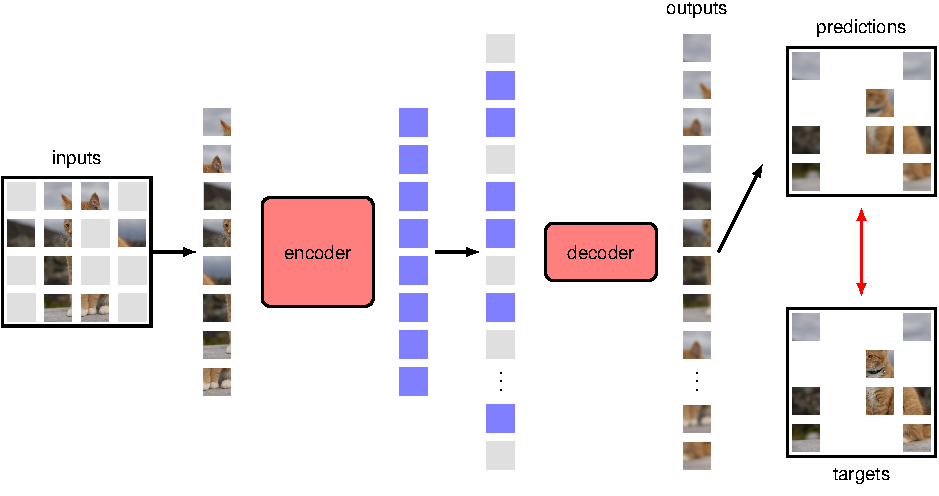
\includegraphics[width=0.8\textwidth]{Figure_5.pdf}
    \end{figure}
\end{frame}

\section{Variational Autoencoders}

\begin{frame}
    \frametitle{Variational autoencoders}
    Because evaluating the likelihood function for a latent-variable model is intractable, the variational autoencoders (VAEs) instead work with an approximation to this likelihood when training the model:
    \begin{itemize}
        \item Use of the evidence lower bound (ELBO) to approximate the likelihood function.
        \item Amortized inference in which a second model, the encoder network, is used to approximate the posterior distributions over latent variables in the E step.
        \item Making the training of the encoder model tractable using the reparameterization trick.
    \end{itemize}
\end{frame}

\begin{frame}
    \frametitle{Evidence lower bound}
    Consider a generative model:
    \begin{itemize}
        \item The distribution over the $M$-dimensional latent variable $z$ is given by a zero-mean unit-variance Gaussian: $p(z)=\mathcal{N}(z;0,I)$.
        \item The conditional distribution $p(x|z;w)$ over the $D$-dimensional data variable $x$ is governed by the output of a deep neural network $g(z;w)$.
    \end{itemize}
\end{frame}

\begin{frame}
    \frametitle{Evidence lower bound}
    We know that for an arbitrary probability distribution $q(z)$ over a space described by the latent variable $z$, we have:
    \begin{align*}
        \log{}p(x;w)&=\mathcal{L}(w)+\mathrm{KL}(q(z)||p(z|x;w))\ge\mathcal{L}(w) \\
        \mathcal{L}(w)&=\int{}q(z)\log\frac{p(x|z;w)p(z)}{q(z)}\mathrm{d}z \\
        \mathrm{KL}(q(z)||p(z|x;w))&=-\int{}q(z)\log\frac{p(z|x;w)}{q(z)}\mathrm{d}z
    \end{align*}
    Although the log likelihood $\log{}p(x;w)$ is intractable, we will seek a way to evaluate $\mathcal{L}(w)$ as an approximation to the true log likelihood.
\end{frame}

\begin{frame}
    \frametitle{Evidence lower bound}
    Now consider a set of training data points $\mathcal{D}=\{x_{1},\hdots,x_{N}\}$, which are assumed to be drawn independently from the model distribution $p(x)$. The log likelihood function for this data set is given by:
    \begin{align*}
        \log{}p(\mathcal{D};w)&=\sum_{n=1}^{N}\mathcal{L}_{n}(w)+\sum_{n=1}^{N}\mathrm{KL}(q_{n}(z_{n})||p(z_{n}|x_{n};w)) \\
        \mathcal{L}_{n}(w)&=\int{}q_{n}(z_{n})\log\frac{p(x_{n}|z_{n};w)p(z_{n})}{q_{n}(z_{n})}\mathrm{d}z_{n}
    \end{align*}
\end{frame}

\begin{frame}
    \frametitle{Evidence lower bound}
    \begin{itemize}
        \item Theorectically, we can set each $q_{n}(z_{n})$ equal to the corresponding posterior distribution $p(z_{n}|x_{n};w)$, which gives zero Kullback-Leibler divergence, and hence the lower bound is equal to the true log likelihood.
        \item However, in practice, exact evaluation of $p(z_{n}|x_{n};w)$ is intractable. We therefore need to find an approximation to the posterior distribution.
    \end{itemize}
\end{frame}

\begin{frame}
    \frametitle{Amortized inference}
    \begin{itemize}
        \item In the variational autoencoder, we train a single neural network, called the encoder network, to approximate all the posterior distributions $p(z_{n}|x_{n};w)$.
        \item The encoder produces a single distribution $q(z|x;\phi)$ that is conditioned on $x$, where $\phi$ represents the parameters of the network.
        \item The objective function, given by the evidence lower bound, now has a dependence on $\phi$ as well as $w$, and we maximize the bound jointly with respect to both sets of parameters.
    \end{itemize}
\end{frame}

\begin{frame}
    \frametitle{Amortized inference}
    A typical choice for the encoder is a Gaussian distribution with a diagonal covariance matrix:
    \begin{equation*}
        q(z|x;\phi)=\prod_{m=1}^{M}\mathcal{N}(z_{m};\mu_{m}(x,\phi),\sigma^{2}_{m}(x,\phi))
    \end{equation*}
\end{frame}

\begin{frame}
    \frametitle{Amortized inference}
    \begin{figure}
        \caption{Illustration of the optimization of the ELBO}
        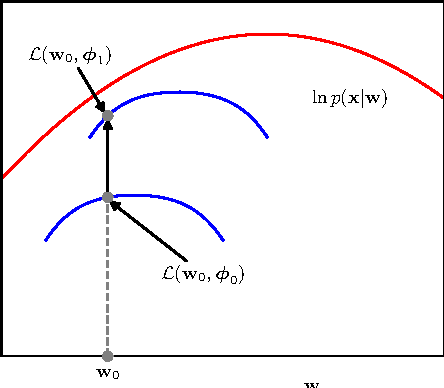
\includegraphics[width=0.4\textwidth]{Figure_8_a.pdf}
        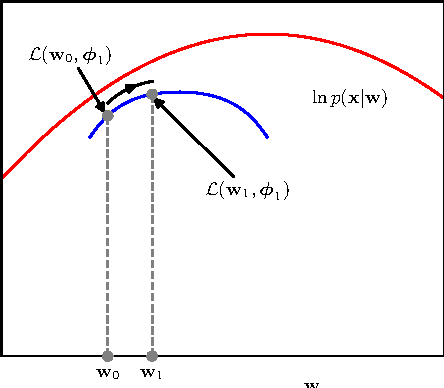
\includegraphics[width=0.4\textwidth]{Figure_8_b.pdf}
    \end{figure}
\end{frame}

\begin{frame}
    \frametitle{Amortized inference}
    \begin{figure}
        \caption{Comparison of the EM algorithm with ELBO optimization in a VAE}
        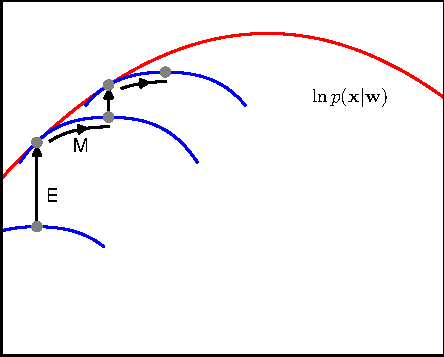
\includegraphics[width=0.4\textwidth]{Figure_9_a.pdf}
        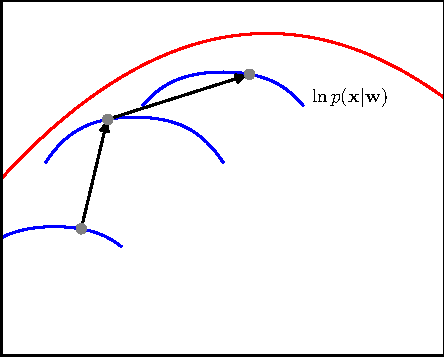
\includegraphics[width=0.4\textwidth]{Figure_9_b.pdf}
    \end{figure}
\end{frame}

\begin{frame}
    \frametitle{The reparameterization trick}
    For data point $x_{n}$, we can write the contribution to the lower bound in the form:
    \begin{align*}
        \mathcal{L}(w,\phi)&=\int{}q(z_{n}|x_{n};\phi)\log\frac{p(x_{n}|z_{n};w)p(z_{n})}{q(z_{n}|x_{n};\phi)}\mathrm{d}z_{n} \\
        &=\int{}q(z_{n}|x_{n};\phi)\log{}p(x_{n}|z_{n};w)\mathrm{d}z_{n}-\mathrm{KL}(q(z_{n}|x_{n};\phi)||p(z_{n}))
    \end{align*}
\end{frame}

\begin{frame}
    \frametitle{The reparameterization trick}
    For the first term, we could try to approximate the intergral over $z_{n}$ with a simple Monte Carlo estimator:
    \begin{equation*}
        \int{}q(z_{n}|x_{n};\phi)\log{}p(x_{n}|z_{n};w)\mathrm{d}z_{n}\approx\frac{1}{L}\sum_{l=1}^{L}\log{}p(x_{n}|z_{n}^{(l)};w)
    \end{equation*}
    where $z_{n}^{(l)}$ are samples drawn from the encoder distribution $q(z_{n}|x_{n};\phi)$. This is easily differentiated with respect to $w$, but the gradient with respect to $\phi$ is problematic.
\end{frame}

\begin{frame}
    \frametitle{The reparameterization trick}
    We can resolve this by making use of the reparameterization trick in which we reformulate the Monte Carlo sampling procedure such that derivatives with respect to $\phi$ can be calculated explicitly. Instead of drawing samples of $z_{n}$ directly, we draw samples from $\mathcal{N}(\epsilon;0,I)$:
    \begin{equation*}
        z_{nm}^{(l)}=\mu_{nm}+\sigma_{nm}\epsilon_{nm}^{(l)}
    \end{equation*}
    where $\mu_{nm}=\mu_{m}(x_{n},\phi)$ and $\sigma_{nm}=\sigma_{m}(x_{n},\phi)$. This makes the dependence on $\phi$ explicit and allows gradients with respect to $\phi$ to be evaluated.
\end{frame}

\begin{frame}
    \frametitle{The reparameterization trick}
    The second term for $\mathcal{L}(w,\phi)$ is a Kullback-Leibler divergence between two Gaussian distributions and can be evaluated analytically:
    \begin{equation*}
        \mathrm{KL}(q(z_{n}|x_{n};\phi)||p(z_{n}))=\frac{1}{2}\sum_{m=1}^{M}(-1-\log\sigma^{2}_{nm}+\mu_{nm}^{2}+\sigma^{2}_{nm})
    \end{equation*}
    The full error function for the VAE, therefore becomes:
    \begin{align*}
        z_{n}^{(l)}&=\mu_{n}+\mathrm{diag}(\sigma_{n1},\hdots,\sigma_{nM})\epsilon_{n}^{(l)} \\
        \mathcal{L}(w,\phi)&=\sum_{n=1}^{N}(\frac{1}{L}\sum_{l=1}^{L}\log{}p(x_{n}|z_{n}^{(l)};w) \\
        &+\frac{1}{2}\sum_{m=1}^{M}(1+\log\sigma^{2}_{nm}-\mu_{nm}^{2}-\sigma^{2}_{nm}))
    \end{align*}
\end{frame}

\begin{frame}
    \frametitle{The reparameterization trick}
    \begin{algorithm}[H]
        \caption{Variational autoencoder training}
        \Repeat{converged}{
            $\mathcal{L}\gets{}0$\;
            \For{$m\gets{}1$ \KwTo $M$}{
                $\epsilon_{nm}\sim\mathcal{N}(\epsilon;0,1)$\;
                $z_{nm}\gets\mu_{nm}+\sigma_{nm}\epsilon_{nm}$\;
                $\mathcal{L}\gets\mathcal{L}+\frac{1}{2}(1+\log\sigma^{2}_{nm}-\mu_{nm}^{2}-\sigma^{2}_{nm})$\;
            }
            $\mathcal{L}\gets\mathcal{L}+\log{}p(x_{n}|z_{n};w)$\;
            $w\gets{}w+\eta\nabla_{w}\mathcal{L}$\;
            $\phi\gets\phi+\eta\nabla_{\phi}\mathcal{L}$\;
        }
        \Return{$w,\phi$}\;
    \end{algorithm}
\end{frame}

\begin{frame}
    \frametitle{The reparameterization trick}
    Problems when training VAEs:
    \begin{itemize}
        \item Posterior collapse: The variational distribution $q(z|x;\phi)$ converges to the prior distribution $p(z)$ and therefore becomes uninformative because it no longer depends on $x$.
        \item Latent code is not compressed.
    \end{itemize}
    Both problems can be addressed by introducing a coefficient $\beta$ in front of the second term in $\mathcal{L}(w,\phi)$ to control the regularization effectiveness of the Kullback-Leibler divergence (\href{https://openreview.net/pdf?id=Sy2fzU9gl}{further references}).
\end{frame}

\end{document}